\documentclass[crop,tikz]{standalone}

\usepackage{makecell}

\definecolor{alizarin}{rgb}{0.82, 0.1, 0.26}
\definecolor{airforceblue}{rgb}{0.36, 0.54, 0.66}
\definecolor{apricot}{rgb}{0.98, 0.81, 0.69}
\definecolor{blush}{rgb}{0.87, 0.36, 0.51}
\definecolor{cadmiumgreen}{rgb}{0.0, 0.42, 0.24}
\definecolor{cambridgeblue}{rgb}{0.64, 0.76, 0.68}
\definecolor{celadon}{rgb}{0.67, 0.88, 0.69}
\definecolor{chestnut}{rgb}{0.8, 0.36, 0.36}
\definecolor{harvardcrimson}{rgb}{0.79, 0.0, 0.09}
\definecolor{darkseagreen}{rgb}{0.56, 0.74, 0.56}
\definecolor{aoenglish}{rgb}{0.0, 0.5, 0.0}
\definecolor{brightube}{rgb}{0.82, 0.62, 0.91}
\definecolor{amethyst}{rgb}{0.6, 0.4, 0.8}
\definecolor{asparagus}{rgb}{0.53, 0.66, 0.42}

\usetikzlibrary{positioning}
\usetikzlibrary{matrix}
\usetikzlibrary{fit}
\usetikzlibrary{calc,decorations.pathmorphing,patterns}
\usetikzlibrary{decorations.pathreplacing}


\newcommand{\vvector}[1]{\tikz{\draw[#1,step=1em,fill=#1!50] (0,0)  grid (1em,4em) rectangle (0, 0);}}
\newcommand{\hvector}[1]{\tikz{\draw[#1,step=1em,fill=#1!50] (0,0)  grid (4em,1em) rectangle (0, 0);}}
\newcommand{\vvectorSmall}[1]{\tikz{\draw[#1,step=.5em,fill=#1!50] (0,0)  grid (.5em,1.5em) rectangle (0, 0);}}

\newdimen\XCoord
\newdimen\YCoord
\newdimen\XXCoord
\newdimen\YYCoord

\newdimen\empty
\newdimen\fromX
\newdimen\fromY
\newdimen\toX
\newdimen\toY

\newcommand{\outgoing}[2]{
  \path (#1); \pgfgetlastxy{\XCoord}{\YCoord};
  \path (#2); \pgfgetlastxy{\XXCoord}{\YYCoord};
  \draw[->, line width=1pt] (\XCoord, \YCoord) -- (\XCoord, \YYCoord);
}%
\newcommand{\incoming}[2]{
  \path (#1); \pgfgetlastxy{\XCoord}{\YCoord};
  \path (#2); \pgfgetlastxy{\XXCoord}{\YYCoord};
  \draw[->, line width=1pt] (\XCoord, \YYCoord) -- (\XCoord, \YCoord);
}%
% horizontal arrow: (#1.x, #3.y) -- (#2.x, #3.y)
\newcommand{\horizontalArrow}[3]{
  \path (#1); \pgfgetlastxy{\fromX}{\empty};
  \path (#2); \pgfgetlastxy{\toX}{\empty};
  \path (#3); \pgfgetlastxy{\empty}{\fromY};
  \draw[->, line width=1pt] (\fromX, \fromY) -- (\toX, \fromY);
}%
% vertical braces: (#3.x, #1.y) -- (#3.x, #2.y)
\newcommand{\verticalBraces}[4]{
  \path (#1); \pgfgetlastxy{\empty}{\fromY};
  \path (#2); \pgfgetlastxy{\empty}{\toY};
  \path (#3); \pgfgetlastxy{\fromX}{\empty};
  % XXX the values for positionning the node for #4 have been choosen for the NMT example. must be checked
  \draw [decorate,decoration={brace,amplitude=3pt,raise=4pt},yshift=0pt] (\fromX, \fromY) -- (\fromX, \toY) node [midway, anchor=west, xshift=.2cm] {#4};
}%


\newcommand{\transformer}{couche encodage}


\begin{document}

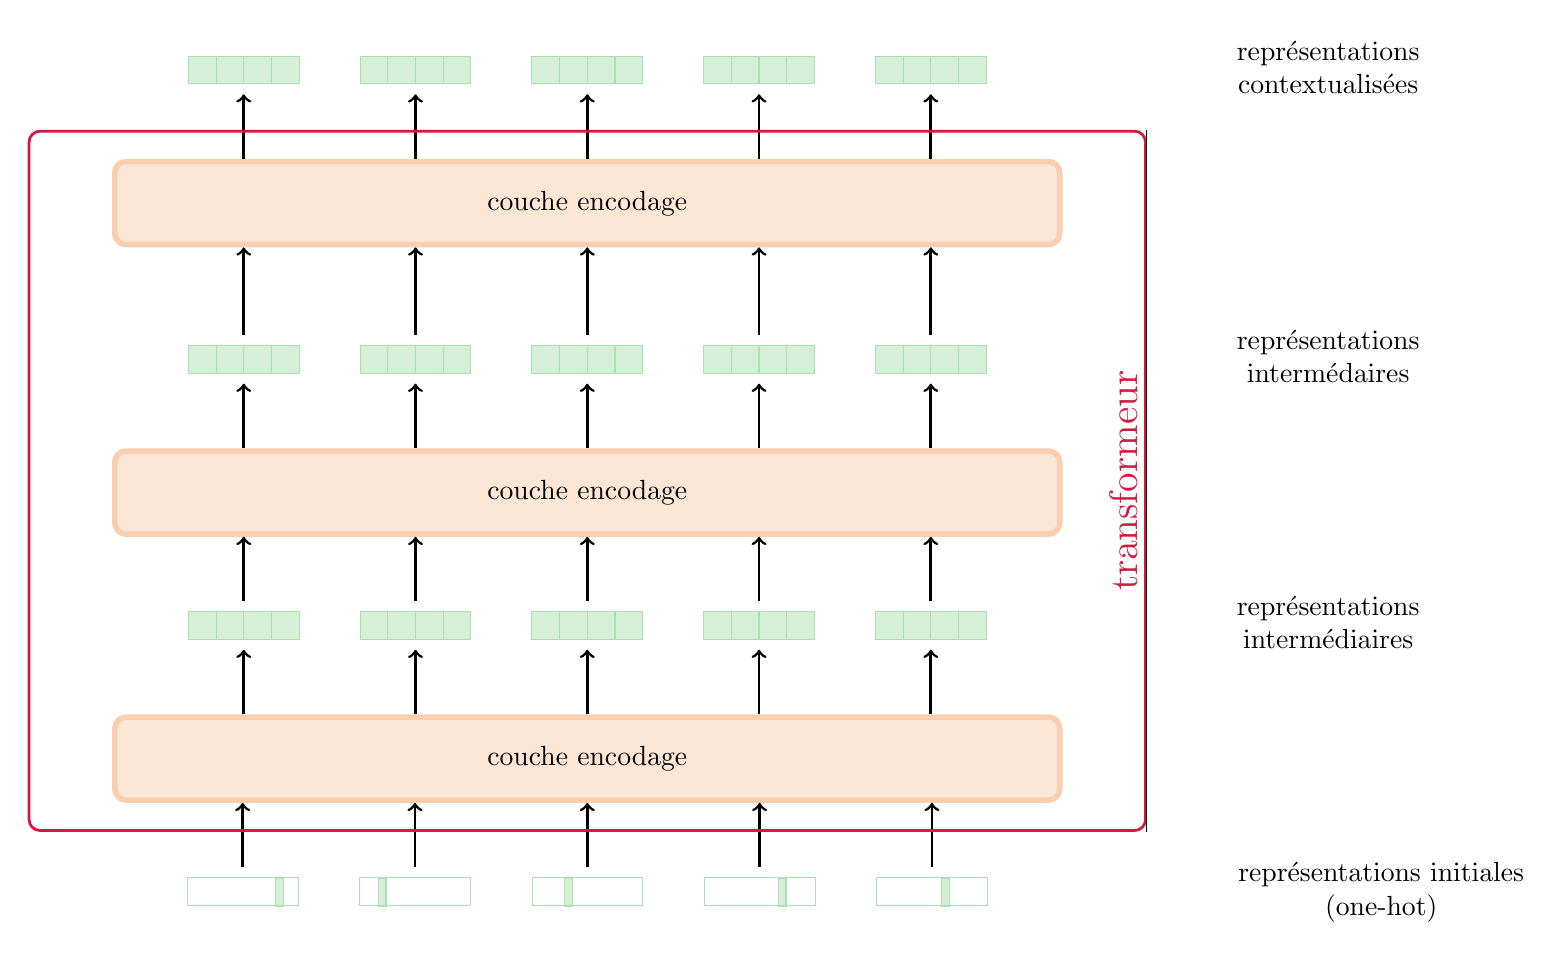
\begin{tikzpicture}[ampersand replacement=\&]

    \node [minimum height=3em, minimum width=12cm, draw=apricot, rounded corners, line width=2pt, fill=apricot!50] (layer1) {\transformer};

    \matrix (repr0) [matrix of nodes,
    column sep=1.5em,
    below=2em of layer1,
    minimum width=2em,]
            { \tikz{\node[draw=celadon, minimum height=1em, minimum width=4em] (w0) at (0, 0) {}; \draw[celadon, fill=celadon!50] (w0.south west) ++(80/100*4em, 0) rectangle ++(0.1, 1em)} \&
              \tikz{\node[draw=celadon, minimum height=1em, minimum width=4em] (w0) at (0, 0) {}; \draw[celadon, fill=celadon!50] (w0.south west) ++(17/100*4em, 0) rectangle ++(0.1, 1em)} \&
              \tikz{\node[draw=celadon, minimum height=1em, minimum width=4em] (w0) at (0, 0) {}; \draw[celadon, fill=celadon!50] (w0.south west) ++(30/100*4em, 0) rectangle ++(0.1, 1em)} \&
              \tikz{\node[draw=celadon, minimum height=1em, minimum width=4em] (w0) at (0, 0) {}; \draw[celadon, fill=celadon!50] (w0.south west) ++(67/100*4em, 0) rectangle ++(0.1, 1em)} \&
              \tikz{\node[draw=celadon, minimum height=1em, minimum width=4em] (w0) at (0, 0) {}; \draw[celadon, fill=celadon!50] (w0.south west) ++(59/100*4em, 0) rectangle ++(0.1, 1em)} \\
            };


    \matrix (repr1) [matrix of nodes,
                      column sep=1.5em,
                      above=2em of layer1,
                      minimum width=2em,]
            { \hvector{celadon} \&
              \hvector{celadon} \&
              \hvector{celadon} \&
              \hvector{celadon} \&
              \hvector{celadon} \\
            };

    \node [above=2em of repr1, minimum height=3em, minimum width=12cm, draw=apricot, rounded corners, line width=2pt, fill=apricot!50] (layer2) {\transformer};

    \matrix (repr2) [matrix of nodes,
    column sep=1.5em,
    above=2em of layer2,
    minimum width=2em,]
            { \hvector{celadon} \&
              \hvector{celadon} \&
              \hvector{celadon} \&
              \hvector{celadon} \&
              \hvector{celadon} \\
            };

    \node [above=of repr2, minimum height=3em, minimum width=12cm, draw=apricot, rounded corners, line width=2pt, fill=apricot!50] (layer3) {\transformer};

    \matrix (repr3) [matrix of nodes,
    column sep=1.5em,
    above=2em of layer3,
    minimum width=2em,]
            { \hvector{celadon} \&
              \hvector{celadon} \&
              \hvector{celadon} \&
              \hvector{celadon} \&
              \hvector{celadon} \\
            };
    
    \foreach \x in {1,...,5} {
        \outgoing{repr0-1-\x.north}{layer1.south};
        \outgoing{repr1-1-\x.north}{layer2.south};
        \outgoing{repr2-1-\x.north}{layer3.south};
        \incoming{repr1-1-\x.south}{layer1.north};
        \incoming{repr2-1-\x.south}{layer2.north};
        \incoming{repr3-1-\x.south}{layer3.north};
    }

    \node[draw=alizarin, rounded corners, line width=1pt, fit=(layer1) (layer3), inner xsep=3em, inner ysep=1em] (box) {};

    \draw (box.north east) -- (box.south east) node[text=alizarin, pos=.5, above, rotate=90] {\Large transformeur};

    \node [right=8em of repr0] {\makecell{représentations initiales \\ (one-hot)}};
    \node [right=8em of repr1] {\makecell{représentations \\ intermédiaires}};
    \node [right=8em of repr2] {\makecell{représentations \\ intermédaires}};
    \node [right=8em of repr3] {\makecell{représentations \\ contextualisées}};

\end{tikzpicture}

\end{document}